\chapter{Exploratory Analysis}
First part of the analysis is to explore the different attributes in the data in order to detect possible patterns or correlations. The exploratory analysis is also used to get an understanding of data and its behaviour. Hence, this chapter is about visualizing the different attributes focusing on their influence on the heat consumption. As the heat in each house is turned off in the summer period, data is segmented such that the summer period is excluded from the data used for modeling. \\

\noindent To get an overview of the heat consumption for each house, the daily average consumption for each house has been calculated and can be seen as a function of the time in figure \ref{fig: daily_cons}. 

\begin{figure}
    \centering
    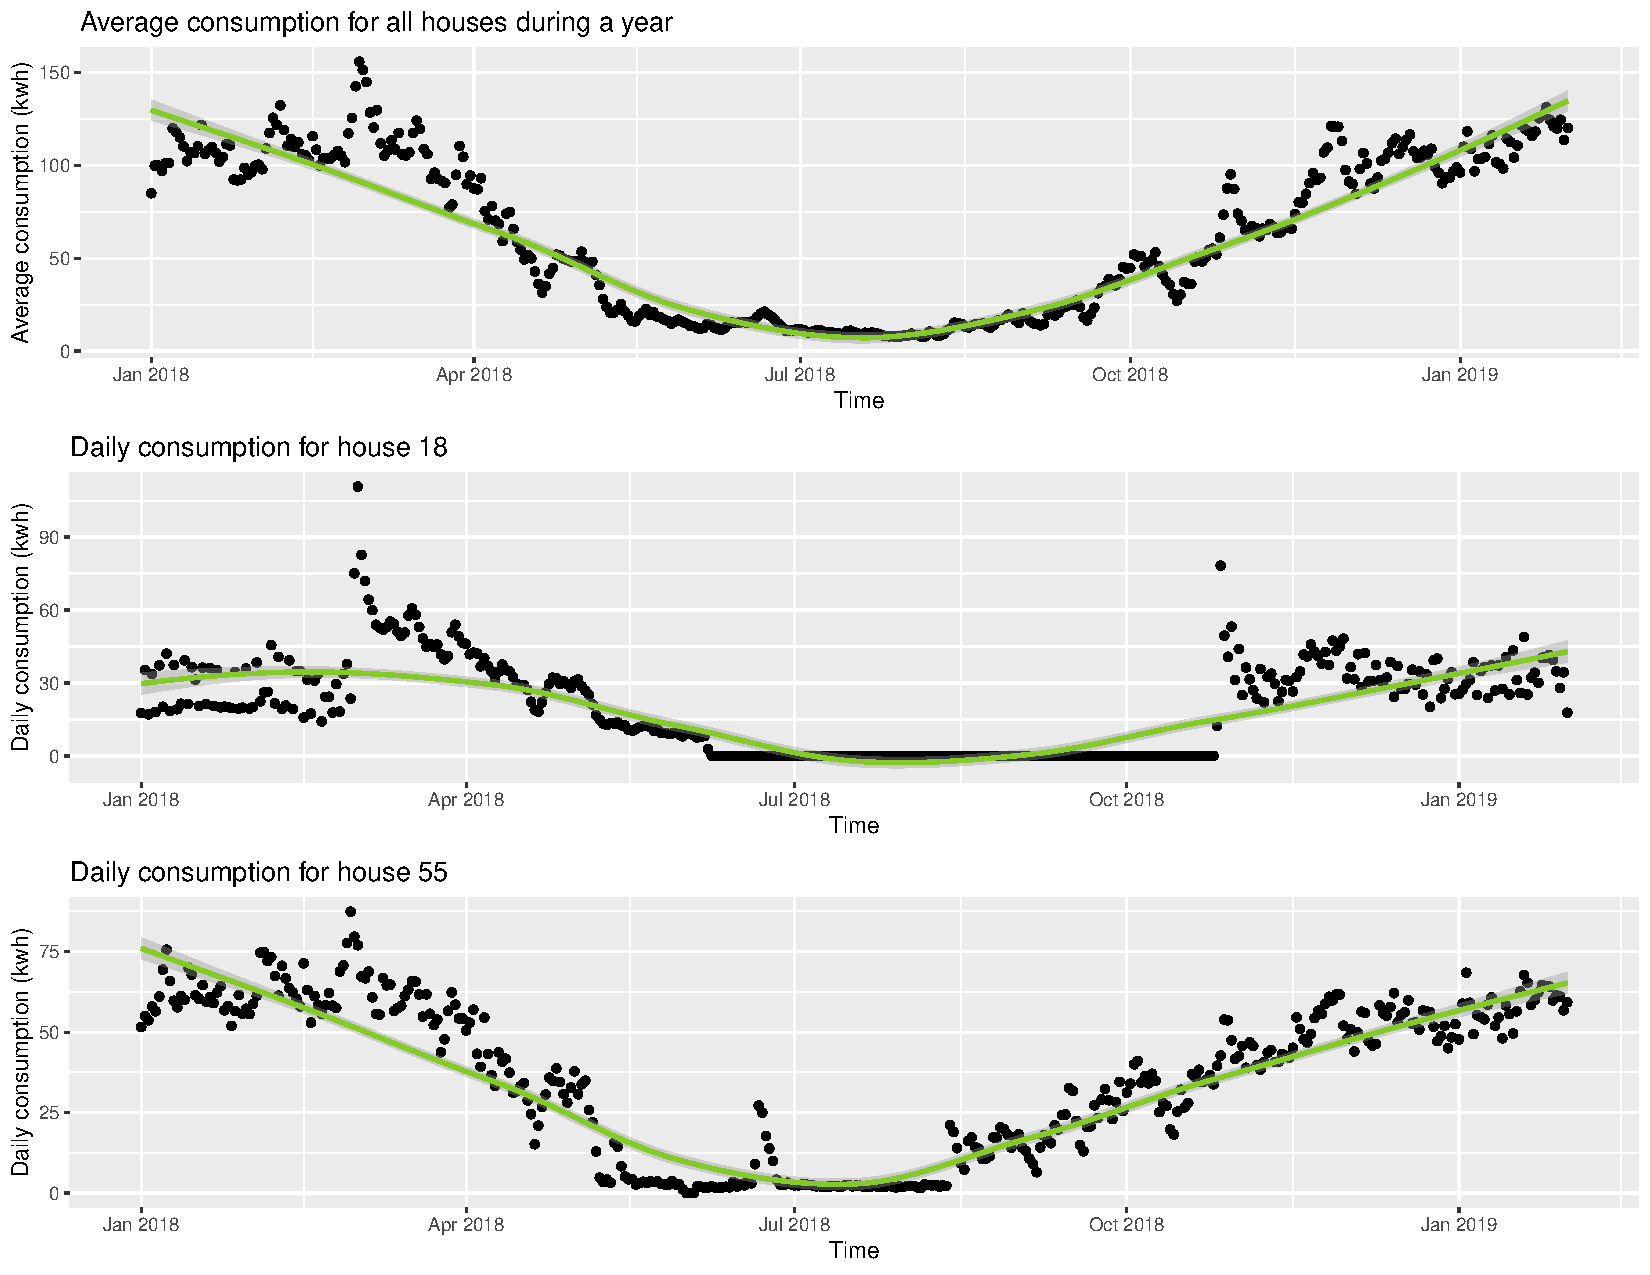
\includegraphics[width=.8\textwidth]{../../../figures/avg_daily.pdf}
    \caption{Daily consumption during a year (2018). The top plot shows the average consumption for all the houses. The plot in the middle shows an example of a house that follows the trend and the last plot shows a house that deviates from the trend}
    \label{fig: daily_cons}
\end{figure}

\noindent Figure \ref{fig: daily_cons} shows the daily average consumption for all the houses and the daily consumption of two houses - one that follows the trend at one that deviates. It can be seen that the slopes around the summer months are close to 0. As mentioned, the data in focus in this project is where the heat is turned on, hence the period where the heat consumption is close to 0 needs to be removed. Exactly how this is done will be explained and discussed in the data segmentation section. All three plots show some unusual high data points around April 2018. This can be due to the fact that is was snowing in Denmark at that time \textcolor{red}{Tilføj reference på det her}. 
\newline \\
\noindent The average of the attributes from the house data is examined through a scatterplot in order to find possible correlations.
\begin{figure}
    \centering
    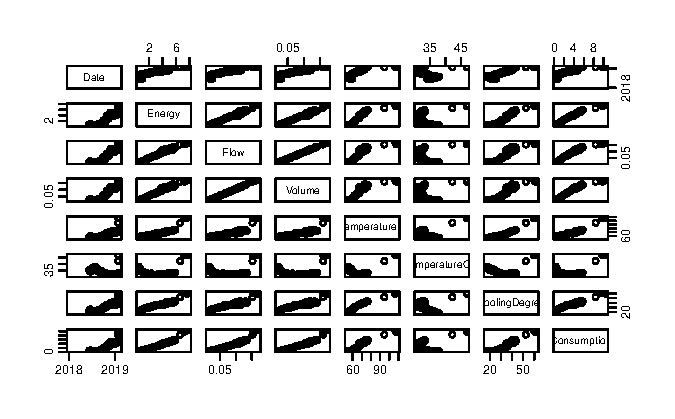
\includegraphics[width=.8\textwidth]{../../../figures/house_attri.pdf}
    \caption{}
    \label{fig: house_attri}
\end{figure}
\noindent Figure \ref{fig: house_attri} clearly shows that the consumption is close to 0 in the summer period.  
\textcolor{red}{Pairs af gennemsnitlig house data - vi ser en masse sammenhænge mellem de forskellige attributer. Vi kan se at CoolingDegree skal være over 25, før at varmeforbruget stiger.}
\textcolor{red}{CoolingDegree begynder at stige et stykke tid før flowet stiger, hvilket hænger godt sammen med at når man fx tænder en radiator så stiger CoolingDegree. De efterfølgende radiatorer man tænder øger volumnet.} \\

\noindent The figure \ref{fig: weather_cons_focus} shows the dependencies between the average consumption of the houses and the weather attributes.
\begin{figure}
    \centering
    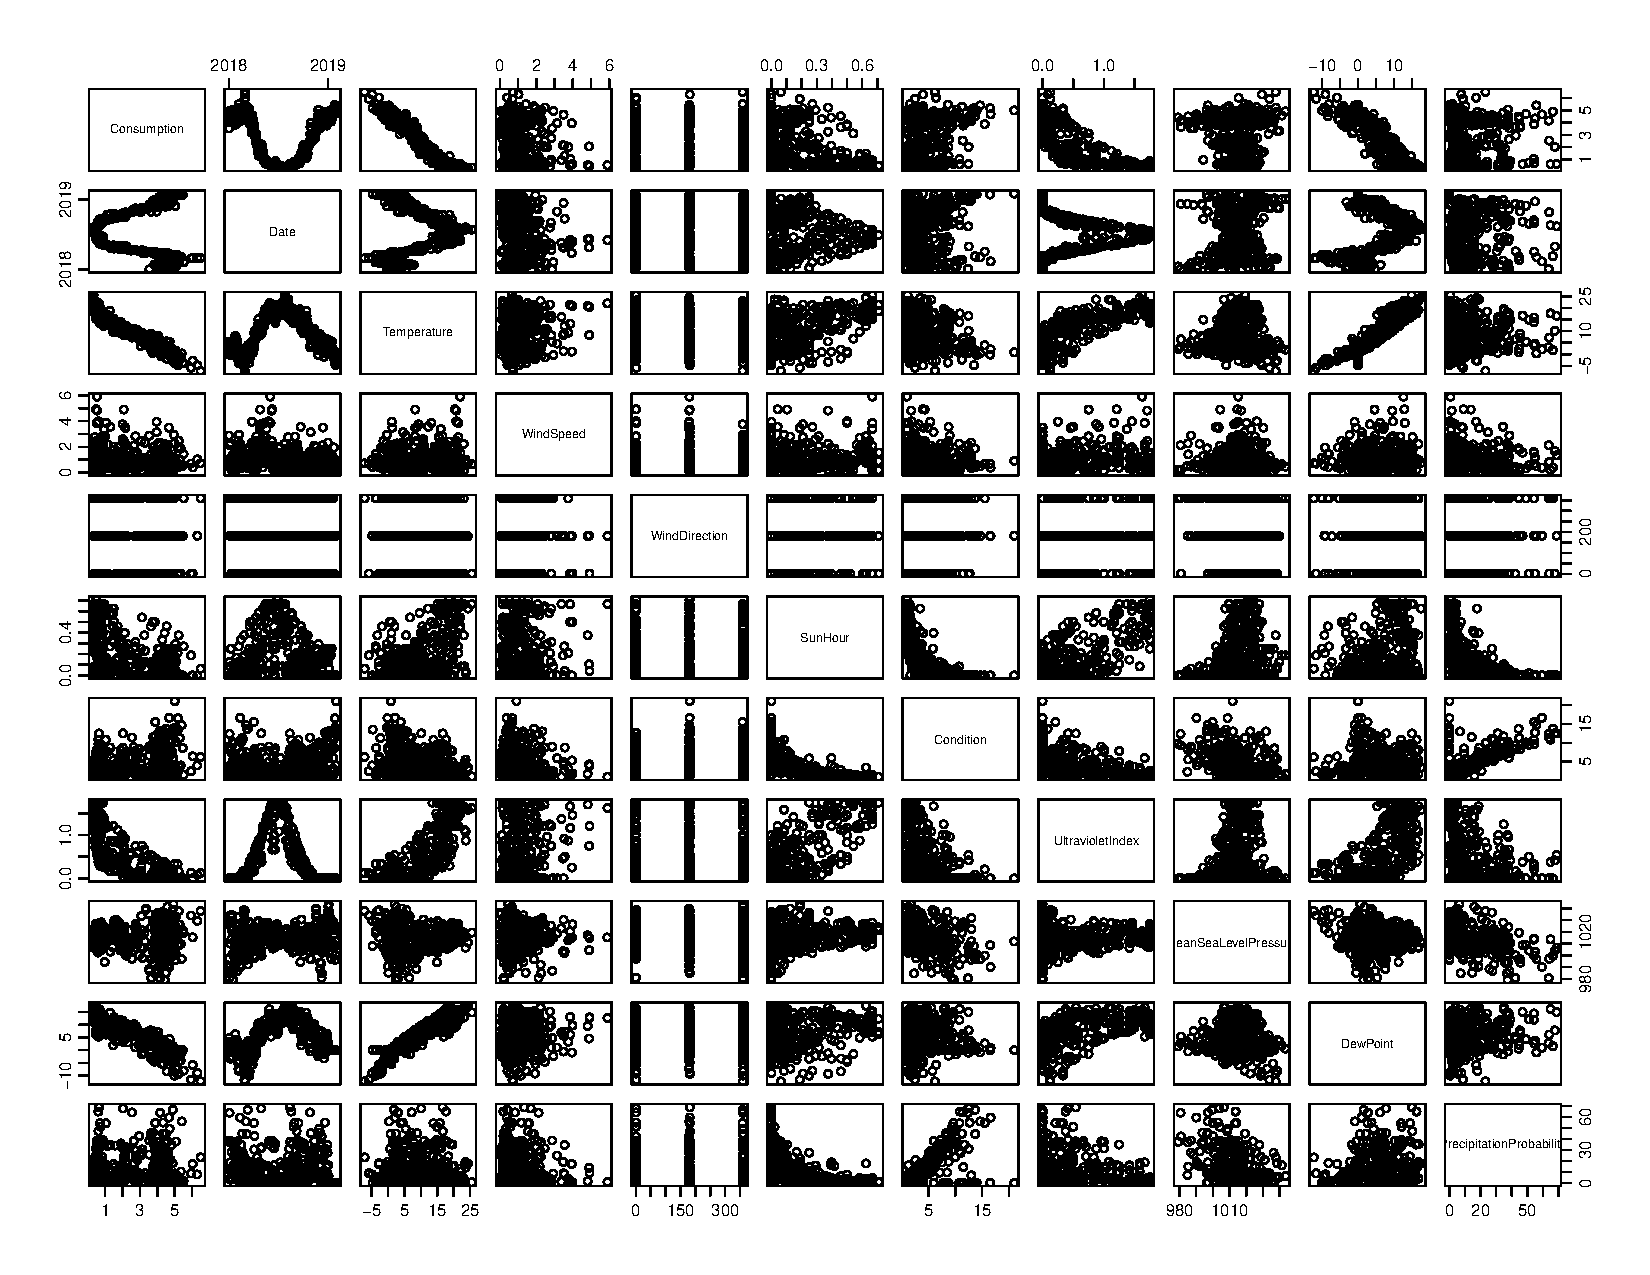
\includegraphics[width=.8\textwidth]{../../../figures/weather_cons.pdf}
    \caption{}
    \label{fig: weather_cons}
\end{figure}

\noindent It is already known that there is a dependency between the heat consumption and the time of year. During the summer period there
is almost no consumption. The consumption in this period is probably mostly tap water. The next important thing is the relation between temperature and consumption. High temperatures tend to imply a higher consumption. And the reason why the consumption depends so clearly on the time of year can be assumed to that certain periods have similar temperature levels. It can also be seen that there is a correlation between dewpoint and consumption. This can be due to the correlation between dewpoint and temperature. \textcolor{red}{Anton nævnte noget med SunHour og Ultravioletindex.}

Figures \ref{fig: house_attri} and \ref{fig: weather_cons_focus}are used to investigate linear relationships which is desired when modeling. If a linear relation is not \textcolor{red}{obtained} this could give rise to a transformation on either the dependent or the independent variable. \textcolor{red}{Jeg synes der mangler lidt her.}

\section{Data segmentation}
Since one of the focuses of this paper is to estimate how much energy a house uses for heating
depending on different outside temperatures, it is important to distinguish between when the house
is actually being heated, and when the water is just being used for tap water consumption. If the
inhabitants are not home for a longer period, there will probably be low consumption, even though
it might be cold outside. This does not necessarily mean that the house is well isolated. And if
there is consumption in warm periods, it is likely to be tap water consumption, and not heating
The data can be seen as part of two different distributions. One where the heating is turned off,
 and one where it is turned on. In this section different approaches will be examined on how to
 distinguish between the two distributions.
The goal is to find some temperature, where it can be assumed that all data points below it belongs
to the distribution with heating turned on. Three approaches will be described below, together with
their pros and cons.

\subsection{Segmentation by piece-wise optimization}
The first approach is to make a linear regression on the data with two segments. A breakpoint
$\alpha$ is found, such that the SSE is as small as possible. The second segment is restricted to
being constant. This way the breakpoint illustrates when the consumption goes from being linearly
dependent on the temperature, to having a constant value. This method was tested on every available
house, where a new breakpoint was found for each house.

\noindent Figure \ref{fig: Consumption-PW} shows the regression for two different houses. On both houses the
line fits rather well with the low-temperature data points. But it is not very accurate around the breakpoint.
The house on the left shows very clearly, that the assumption that all points below the breakpoint belong to 
the distribution without heating, is not accurate. Even though this approach can easily take out a lot of data
where there is clearly no heating, it will in many cases set the breakpoint too high. The "tail" of the low
consumption distribution might still be included, causing a bias in the model, and some variation that is not
accounted for. The method is also not very robust. Depending on how the points are spread out, the breakpoint
is sometimes as high as 20 degrees, which is not desirable.
\begin{figure}
    \centering
    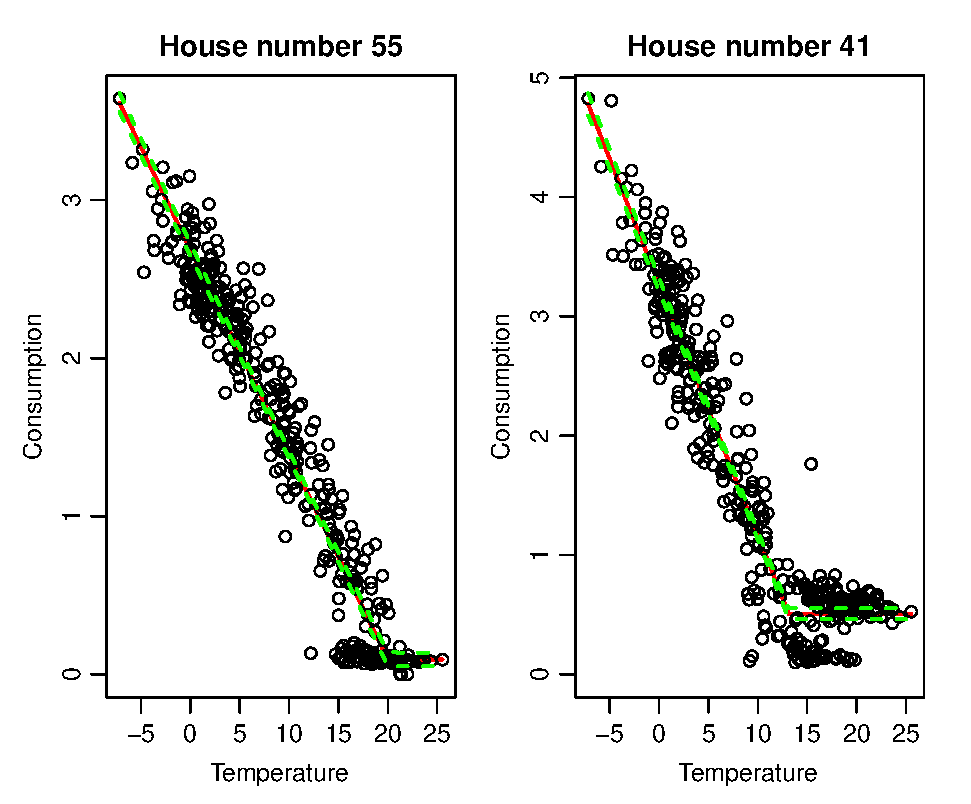
\includegraphics[width=0.8\textwidth]{../../../figures/Consumption-PW.eps}
    \caption{Piece-wise optimization of the consumption. The red line is the regression line and the green line is the confidence interval.}
    \label{fig: Consumption-PW}
\end{figure}

\subsection{Segmentation by investigation slopes}


\subsection{Segmentation by significant deviations}
In the third approach, the data points are examined from high temperatures to low. First, all data points from
above 20 degrees are assumed to belong to the distribution without heating. Using this data set, an interval
of two standard deviations is calculated. For each degree interval, starting from above and moving down, all
data points in that interval are examined. If more than 80\% of them are outside the two standard deviations,
the upper bound of that degree interval is used as the segmentation breakpoint.


\begin{figure}
    \centering
    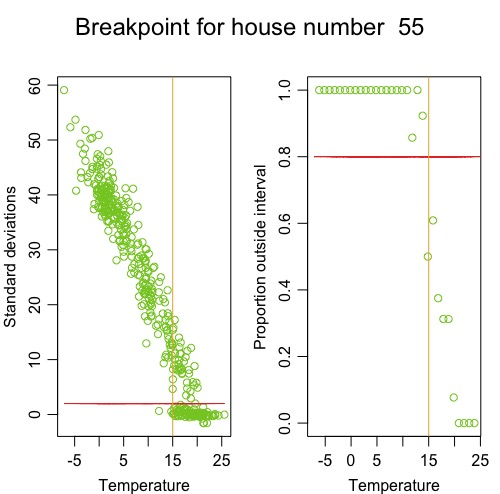
\includegraphics[width=0.8\textwidth]{../../../figures/Breakpoint.jpeg}
    \caption{Piece-wise optimization of the consumption. The red line is the regression line and the green line is the confidence interval.}
    \label{fig: Consumption-PW}
\end{figure}


%\subsection{Bestemmelse af temperatur breakpoint:}
%\begin{itemize}
%    \item Vi kigger på de huse der har mindst et års data (så vi er sikker på at hele sommeren er med)
%    \item Vi antager at dagene med over 20 grader udenfor, der er der slukket for varmen, og der er dermed kun varmvandsforbruget med, som vi antager er hvid støj.
%    \item For hver grad under 20 ser vi hvor mange procent af consumptionen der ligger indenfor +-2 standardafvigelser fra 20+ sættet.
%    \item Den første grad hvor mere end 20\% af datapunkterne ligger indenfor intervallet gemmes som det hus' alpha.
%    \item vi tager til sidst 15\% "percentile" af alphaerne, og skærer alt data fra vores datasæt som er over 12 grader.
%\end{itemize}

\section{BBR data}

\begin{figure}
    \centering
    \includegraphics[width=.8\textwidth]{../../../figures/byggeår.eps}
    \caption{}
    \label{fig: byggeår}
\end{figure}

\begin{itemize}
    \item Vi tager gennemsnittet af consumption over alle dage under 12 grader for hvert hus.
    \item Dette bliver divideret med det samlede boligareal.
    \item Når dette gøres ses 1 tydelig outlier, der tilhører en lejlighed på 61 $m^2$ bygget i 1920.
    \item Når vi plotter gennemsnitsconsumption med det seneste ombygningsår, ser vi en tendens af, at jo senere huset er blevet bygget om, jo mindre er varmeforbruget for huset.
\end{itemize}    

\section{Multicollinearity}
Multicollinearity occurs when two or more explanatory variables are highly correlated. In linear regression, multicollinearity \textcolor{red}{\dots} 
\begin{table}
    \centering
    \begin{tabular}{ll}
     \hline
     \textbf{Attributes} & \textbf{Correlation}  \\
    \hline
    \hline
    Temperature \& DewPoint  &  0.936 \\
    Temperature \& UltraVioletIndex  & 0.611 \\
    PrecipitationProbability \& Condition & 0.826 \\
    \hline
    \end{tabular}
    \caption{Correlation between explanatory variables selected based on figures \ref{fig: house_attri}-\ref{fig: weather_cons}}
    \label{tab: correlation_table}
\end{table}   
Table \ref{tab: correlation_table} clearly shows that the attributes temperature and dewpoint are highly correlated as their correlation is close to 1. Hence, it is decided to remove the attribute \texttt{DewPoint} while \texttt{Temperature} is kept. The correlation between \texttt{PrecipitationProbability} and \texttt{Condition} are also quite high. However, it is decided to keep both of the attributes since \textcolor{red}{...} \\

\noindent The complete data set used for modeling in chapter 4 can be seen in table \ref{tab: modeldata} 
\begin{table}
    \centering
    \begin{tabular}{ll}
     \hline
     \textbf{Variable} & \textbf{Description} \\
    \hline
    \hline
    Date  &  End time and date for measurements. Hourly values.\\
    Temperature  &  Temperature outside in Degrees/C. \\
    WindSpeed  &  \\
    WindDirection  &  \\
    SunHour  &  \\
    Condition  & \\
    UltravioletIndex  &   \\
    MeanSeaLevelPressure  & \\
    PrecipitationProbability & \\
    Observation & The number of observations for each day for each house.\\
    Consumption & CoolingDegree times Volume from House data \\
    Holiday & \\
    \hline
    \end{tabular}
    \caption{Attributes used for modelling.}
    \label{tab: modeldata}
\end{table}   